% Updated by Michael Gertz, April 2017
%%%%%%%%%%%%%%%%%%%%%%%%%%%%

\documentclass{beamer}
%\usepackage[ngerman]{babel}
\usepackage[utf8]{inputenc}

\usepackage{color}
\usepackage{graphicx}
\usepackage{fancybox}

\usepackage{forest}
\usepackage{listings}

\definecolor{dkgreen}{rgb}{0,0.6,0}
\definecolor{mauve}{rgb}{0.58,0,0.82}

\lstdefinestyle{myCustomMatlabStyle}{
	language=C,
	numbers=left,
	stepnumber=1,
	numbersep=10pt,
	keywordstyle=\color{blue},
	commentstyle=\color{dkgreen},
	tabsize=4,
	showspaces=false,
	showstringspaces=false
}

\usepackage{beamerthemesplit}
\usetheme[compress]{Heidelberg}
\definecolor{unirot}{rgb}{0.5976525,0,0}
\usecolortheme[named=unirot]{structure}


\title[IR with PostgreSQL]{Information Retrievel with PostgreSQL}
\author[Alexander Hebel]{Alexander Hebel}
\date{Mai 6, 2020}
\institute[Uni HD]{
Heidelberg University\\
Institute of Computer Science\\
Database Systems Research Group\\
\color{unirot}{vx228@uni-heidelberg.de}}

%---------------------------------------%
%---------- RECURRING OUTLINE ----------%
% have this if you'd like a recurring outline
\AtBeginSection[]  % "Beamer, do the following at the start of every section"
{
\begin{frame}<beamer> 
\frametitle{Outline} % make a frame titled "Outline"
\tableofcontents[currentsection,hideallsubsections]  % show TOC and highlight current section
\end{frame}
}
%----------------------------------------


\begin{document}
\frame[plain]{\titlepage}
\frame{\frametitle{Outline}\tableofcontents[hideallsubsections]}

%========================================
%========================================

\section[Introduction]{Introduction}

\subsection{Introduction}


\frame{
\frametitle{Information Retrieval System (IRS)}

\begin{block}{\centering Information Retrieval (IR)}
	\begin{itemize}
		\item Information retrieval is the science of searching for information in a document		
		\item An IR system is a software system that provides access to books, journals and other documents; stores and manages those documents. 
		\item Web search engines are the most visible IR applications.
	\end{itemize}
\end{block}

\begin{block}{\centering Full-Text-Search}
	The activity of searching through a collection of natural-language documents to locate those that best match a query
\end{block}

}

	
\frame{	
\frametitle{Objectives}

	\begin{block}{}
		IRS already exist.\\
		But to our best knowledge there is no IRS made of a relational database.
	\end{block}

	\begin{itemize}
		\item Finding different sutiable database models
		\item Python api for the database creation and communication
		\item Crawl Wikipages to gather text data
		\item Store and manage those text documents 
		\item Support search querys with the boolean operator AND
		\item Create a ranking function for the query results
		\item Compare the ranking of whole wiki pages and their sections
	\end{itemize}
} % END OF FRAME


\frame{	
	\frametitle{Tsvector and Tsquery}
	
	\begin{itemize}
		\item PostgreSQL provides \textbf{two} data types that are designed to support full text search
		\item The \textbf{tsvector} type represents a document in a form optimized for text search
		\item The \textbf{tsquery} type similarly represents a text query
	\end{itemize}

	\begin{block}{\centering Example Tsvector}
		SELECT to\_tsvector('english', 'The Fat Rats');\\
		\{'fat':2 'rat':3\}
	\end{block}

	\begin{block}{\centering Example Tsquery}
		SELECT to\_tsquery('Fat:ab \& Cats');\\
		\{'fat':AB \& 'cat'\}
	\end{block}
} % END OF FRAME

%========================================
%========================================

\section[Realization]{Approach and Realizations}

\subsection{Approach and Realizations}

\frame{
	\frametitle{Realization}
	
	\begin{block}{\centering Wiki crawler}
		\centering
		\begin{itemize}
			\item Based on package wikipedia version 1.4.0
			\item Takes number of pages and category as input 
			\item Also searches in subcategories
			\item Variable level of subcategories
		\end{itemize}
	\end{block}

	\begin{block}{\centering Database pipeline}
		\centering
		\begin{itemize}
			\item Used package psycopg2 version 2.8.5
			\item Custom converter for tsvector
		\end{itemize}
	\end{block}

	\begin{block}{\centering Document Definition}
		A document in my case is either a page title, seciton title or section text
	\end{block}
} % END OF FRAME

\frame{	
	\frametitle{Text Data Statistics}
	
	\begin{block}{\centering Wikipedia Category "Sports"}
		\centering
		\begin{itemize}
			\item Number of Wiki pages: 2000
			\item Number of sections (captions also count as section): 45756
			\item Total number of words: 17587832
			\item Total number of lexemes: 1969427
		\end{itemize}
	\end{block}

	\begin{block}{}
		\begin{itemize}
			\item Max number of words of a page: 124136
			\item Max number of lexemes of a page: 17787
		\end{itemize}
	\end{block}

	\begin{block}{}
		\begin{itemize}
			\item Max number of words of a section: 24163
			\item Max number of lexemes of a section: 2785
			\item Average number of words per section: 734.7
		\end{itemize}
	\end{block}
} % END OF FRAME

\frame{	
	\frametitle{Text Data Statistics 2}
	
	\begin{block}{\centering Top 10 Frequent Terms}
		\begin{itemize}
		\item[(1)] "game" \qquad \qquad TF: 14044 \quad DocF: 5370
		\item[(2)] "world" \qquad \qquad TF: 13568 \quad DocF: 6144
		\item[(3)] "championship" $\>$ TF: 12106 \quad DocF: 5475
		\item[(4)] "team" \qquad \quad $\>$ $\>$ TF: 11955 \quad DocF: 4362
		\item[(5)] "sport" \qquad \quad $\>$ $\>$ TF: 10658 \quad DocF: 5014
		\item[(6)] "1" \qquad \quad \qquad $\>$ TF: 10237 \quad DocF: 4029
		\item[(7)] "first" \qquad \qquad $\>$ TF: 10199 \quad DocF: 5073
		\item[(8)] "player" \qquad $\>$ $\>$ $\>$ TF: 9577 $\>$ \quad DocF: 3243
		\item[(9)] "2" \qquad \qquad \quad $\>$ TF: 9090 $\>$ \quad DocF: 3821
		\item[(10)] "play" \quad $\>$ $\>$ $\>$ $\>$ $\>$ $\>$ TF: 9082 $\>$ \quad DocF: 3827
	\end{itemize}
	TF = term frequency \qquad DocF = document frequency
	\end{block}
}

\frame{
\frametitle{Three Database Model Approaches}

\begin{columns}[t]
	\begin{column}{.33\textwidth}
		{\color{unirot}Tsvector}
		\begin{block}{}
			\centering
			\begin{itemize}
				\item full text search with tsvector
				\item ranking function of tsvector
				\item weighting of tsvector
				\item tokenization and lemmatization
				\item tsquery
			\end{itemize}
		\end{block}	
	\end{column}
	
	\begin{column}{.33\textwidth}
		{\color{unirot}Mix} 
		\begin{itemize}
			\item raw tsvector + word-matrix for each doc
			\item needs a lot of memory
			\item customizable
		\end{itemize}
	\end{column}

	\begin{column}{.33\textwidth}
		{\color{unirot}Word-matrix} 
		\begin{itemize}
			\item one big word-matrix
			\item probably slow
		\end{itemize}
	\end{column}
\end{columns}
\vfill
} % END OF FRAME

\frame{
\frametitle{Database model}

\begin{figure}
	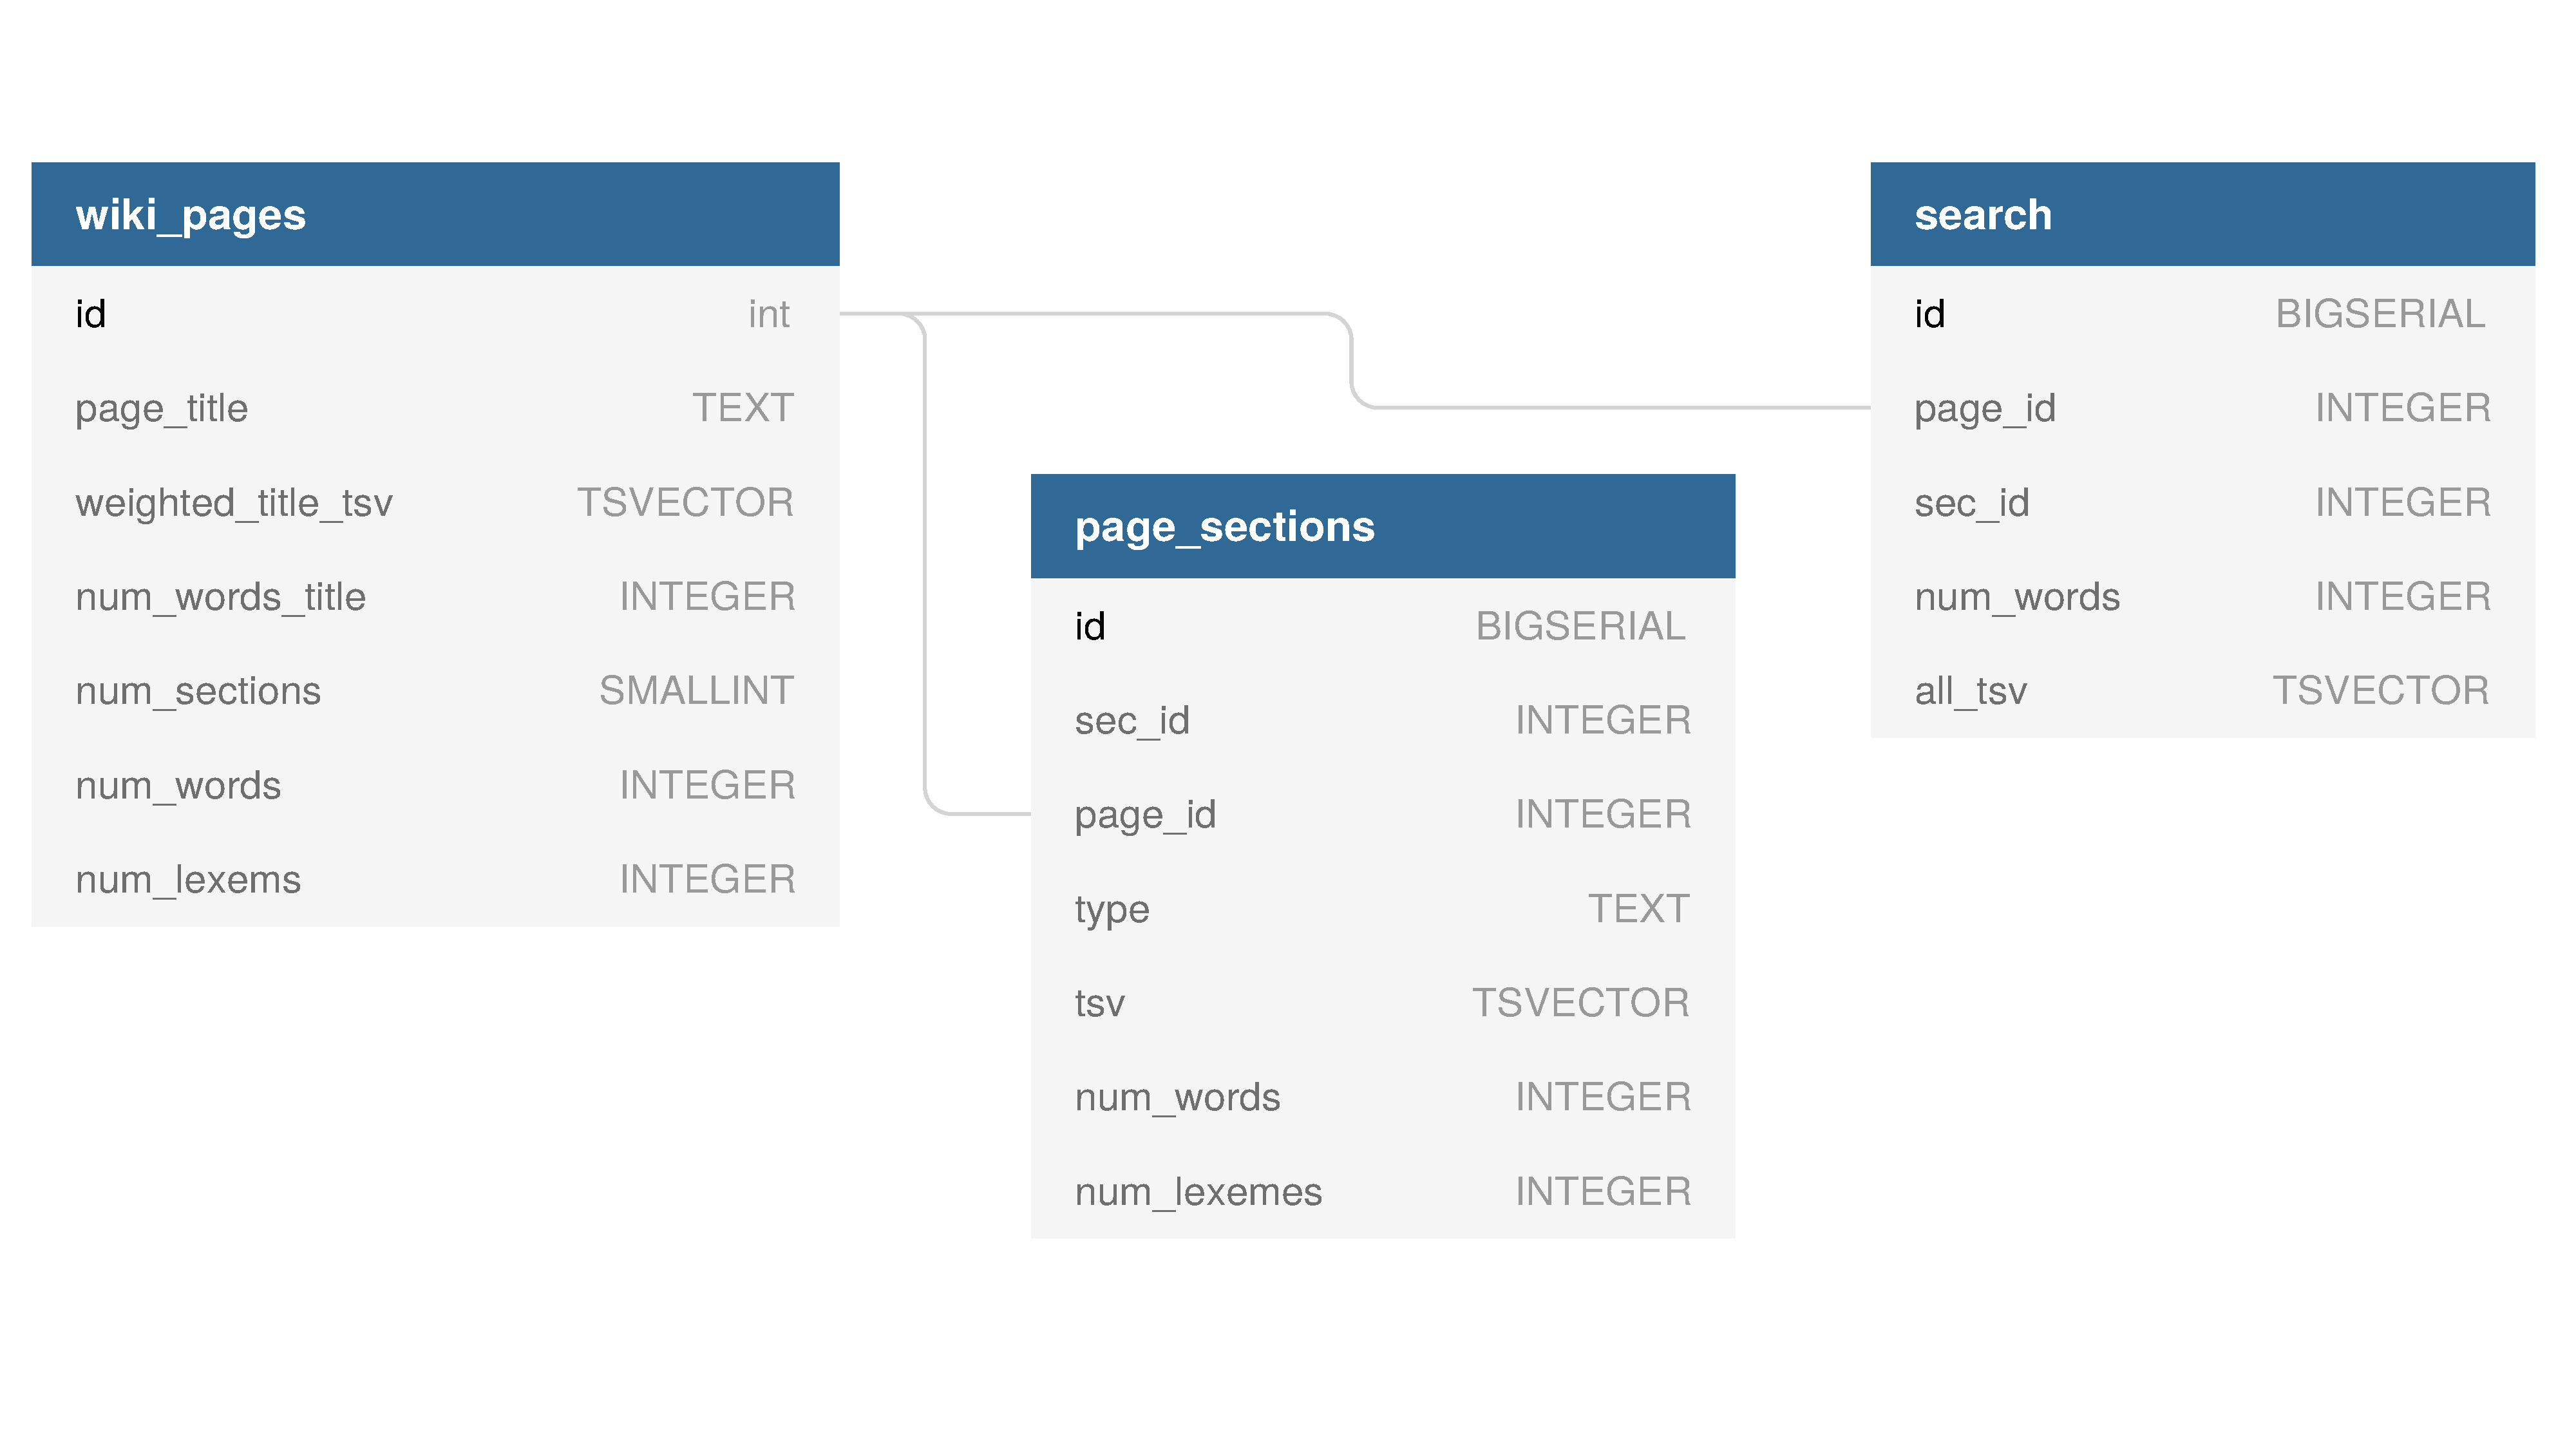
\includegraphics[width=1.\textwidth]{db_scheme} 
\end{figure}

} % END OF FRAME

\frame{
	\frametitle{Tsvector}
	
	\begin{columns}[t]
		\begin{column}{.5\textwidth}
			{\color{unirot}Possibilities}
			\begin{itemize}
				\item Full text search
				\item GIN-Index
				\item Automatic tokenization and lemmatization
				\item Adding weights
				\item Predefined ranking function
			\end{itemize}
		\end{column}	
		
		\begin{column}{.5\textwidth}
			{\color{unirot}Limitations} 
			\begin{itemize}
				\item The number of lexemes must be less than $2^{64}$ 
				\item Max position value: 16383
				\item No more than 256 positions per lexeme
				\item Relative small set of manipulation methods
				\item Ranking function must be customized
			\end{itemize}
		\end{column}
	\end{columns}	
} % END OF FRAME


%========================================
%========================================

\section[Customize Tsvectors]{Adding Functionality to Tsvectors}

\subsection{Adding Functionality to Tsvectors}

%----------------------------------------

\def\hilite<#1>{%
  \temporal<#1>{\color{black}}{\color{unirot}}%
               {\color{gray}}}
               
%----------------------------------------


\frame{
	\frametitle{Reason to Extend PostgreSQL}
	
	\begin{block}{}
		\centering
		Only a few manipulation methods for tsvectors exist
	\end{block}

	For example it is not possible to:
	
	\begin{itemize}
		\item[-] count the occurrence of \textbf{all} lexemes in a tsvector \\ (not only the number of distinct lexemes)
		\item[-] create a tsvector with an offset for the position index
		\item[-] get the max index of a tsvector
		\item[-] concatenate two tsvecotrs without changing the position values
	\end{itemize}

	\begin{block}{\centering Solution}
		\centering
		Write your own function either in plpgsql language or in C 
	\end{block}
	
}


\frame{
\frametitle{Custom C-Functions in PostgreSQL}

\begin{columns}[t]
	\begin{column}{.5\textwidth}
		{\color{unirot}Prerequisites}
		\begin{itemize}
			\item Developer version of PostgreSQL
			\item Installation of make
			\item Root privilege on database
		\end{itemize}
	\end{column}
	
	
	\begin{column}{.5\textwidth}
		{\color{unirot}Folder structure} 
		\begin{forest}
			for tree={
				font=\ttfamily,
				grow'=0,
				child anchor=west,
				parent anchor=south,
				anchor=west,
				calign=first,
				edge path={
					\noexpand\path [draw, \forestoption{edge}]
					(!u.south west) +(7.5pt,0) |- node[fill,inner sep=1.25pt] {} (.child anchor)\forestoption{edge label};
				},
				before typesetting nodes={
					if n=1
					{insert before={[,phantom]}}
					{}
				},
				fit=band,
				before computing xy={l=15pt},
			}
			[Extension
			[function.c]
			[Makefile]
			[function.control]
			[function--1.0.sql]
			[README.function]
			]
		\end{forest}
	\end{column}
\end{columns}
\vfill
\begin{block}{\centering Steps}
	\begin{itemize}
		\item[(1)] make install
		\item[(2)] CREATE EXTENSION "extension"
	\end{itemize}
\end{block}
} % END OF FRAME

%========================================
%========================================

\section[Evaluation Objectives]{Evaluation Objectives}

\subsection{Evaluation Objectives}

\frame{
\frametitle{Evaluation Objectives}

\begin{itemize}
	\item Three different database models have been implemented
	\item The model mainly using tsvector has proven most suitable
	\item[+] GIN index for performance
	\item[+] ts\_rank() function for ranking
	\item[+] ts\_query even supports phraseto\_tsquery()
\end{itemize}

\begin{block}{\centering Calculation of Ranking}
	\begin{itemize}
		\item[-] Either with ts\_rank() or Cover Density Ranking (CDR)
		\item[-] Considers word occurrences and distance between words
	\end{itemize}
\end{block}

\begin{block}{\centering Relationship Between Page and Section Ranking}
	\begin{itemize}
		\item \textbf{section ranking}: ranking / num\_words\_of\_section
		\item \textbf{page ranking}: sum\_of\_rankings / num\_words\_of\_page
	\end{itemize}
\end{block}

}

\frame{
	\frametitle{Query:"game", Sorted by Sum of Section Rankings}
	
	\begin{figure}
		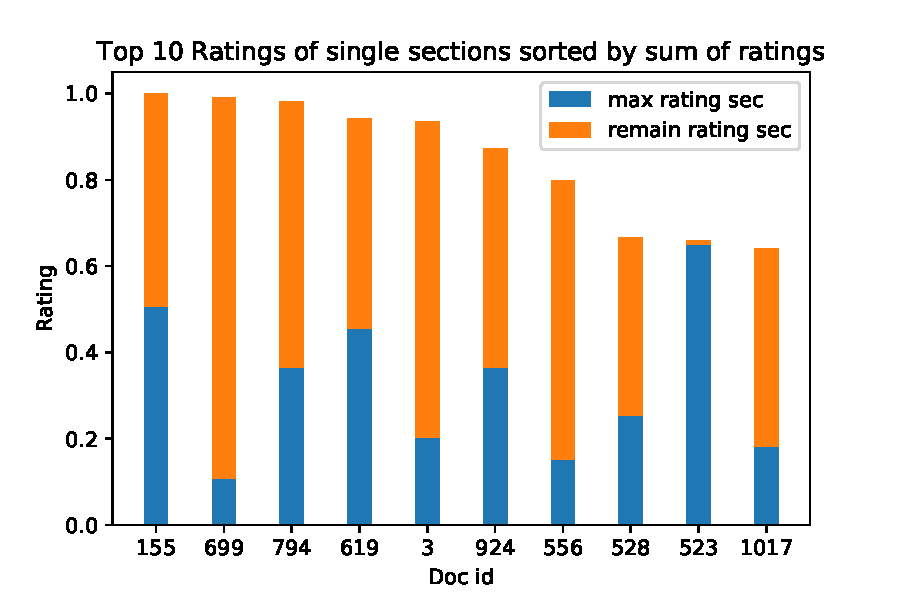
\includegraphics[width=1.\textwidth]{2000_only_sec_sorted_by_sum} 
	\end{figure}
}

\frame{
	\frametitle{Query:"game", Adding The Rank for the Whole Page}
	
	\begin{figure}
		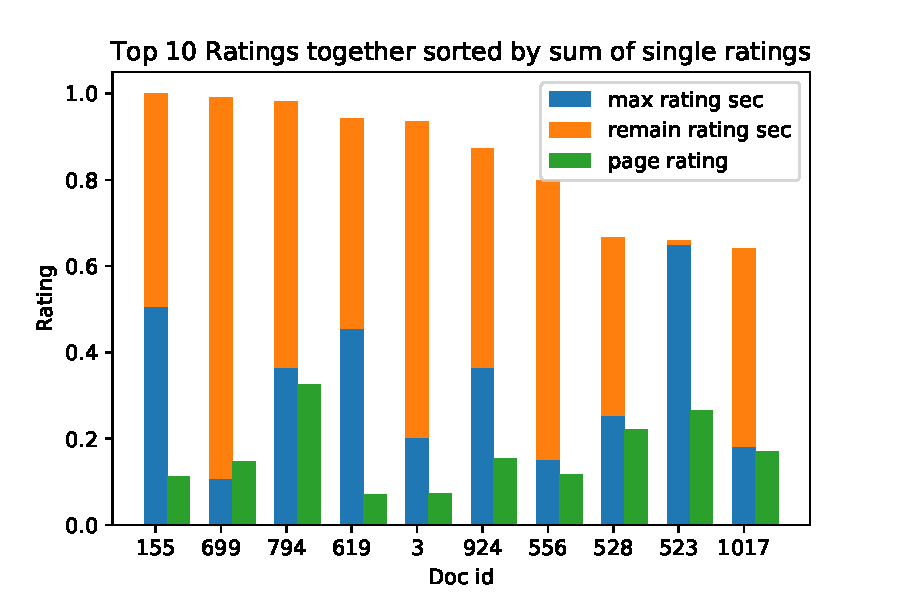
\includegraphics[width=1.\textwidth]{2000_together_sroted_by_sum} 
	\end{figure}
}

\frame{
	\frametitle{Query:"game", Ordered by Max Section Ranking}
	
	\begin{figure}
		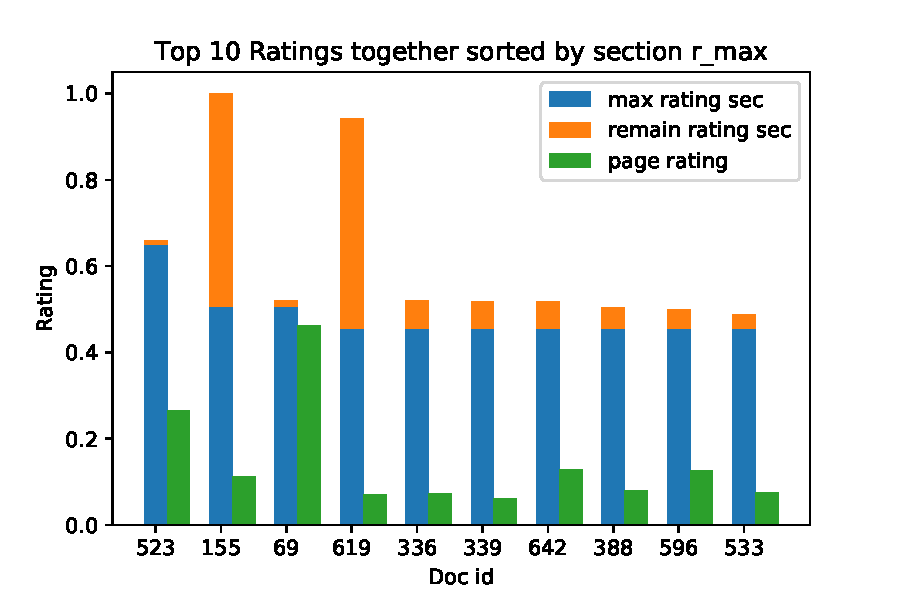
\includegraphics[width=1.\textwidth]{ordered_by_rmax_together} 
	\end{figure}
}

\frame{
	\frametitle{Query:"game AND team AND ball", Ordered by Max Section Ranking}
	
	\begin{figure}
		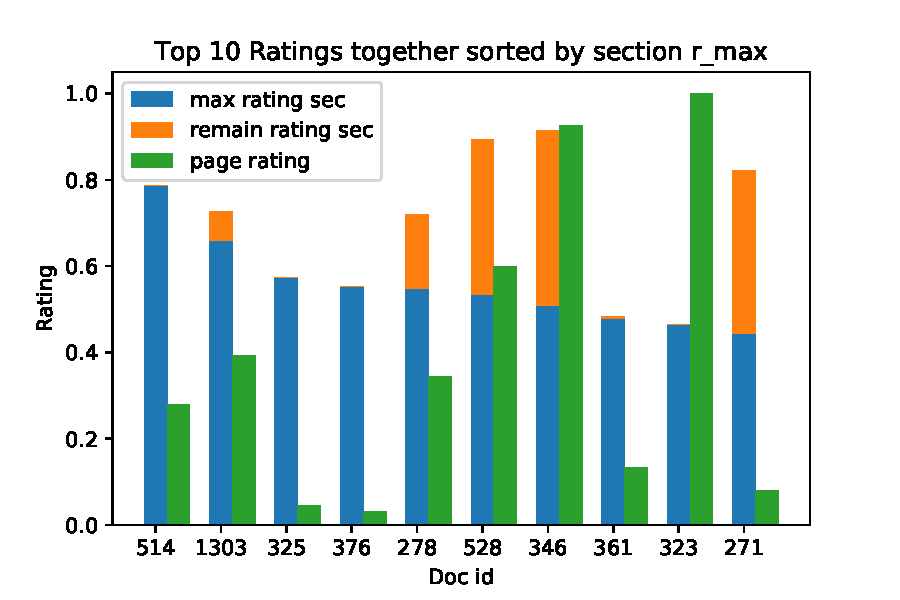
\includegraphics[width=1.\textwidth]{tripel_ordered_by_rmax_together} 
	\end{figure}
}

\frame{
	\frametitle{Distance Between Rankings}
	
	\begin{block}{\centering Calculating Distance}
		\begin{itemize}
			\item To calculate the difference between pageranking and sectionranking
			\item Distance first of max section rank to first of max page rank, distance of second max section ranking to second of max page rank and so on...
		\end{itemize}
	\end{block}
	
	\begin{columns}[t]
		\begin{column}{.5\textwidth}
			{\color{unirot}Query "game"}
			\begin{itemize}
				\item result pages: 1176
				\item Top 10 - 289.5 avg(dist) 
				\item Top 20 - 250.9 avg(dist) 
				\item Top 30 - 183.2 avg(dist) 
				\item Top 40 - 155.5 avg(dist) 
			\end{itemize}
		\end{column}
		
		
		\begin{column}{.5\textwidth}
			{\color{unirot}Query "game \& team \& ball"} 
			\begin{itemize}
				\item result pages: 274
				\item Top 10 - 36.0 avg(dist)
				\item Top 20 - 40.6 avg(dist)
				\item Top 30 - 36.6 avg(dist)
				\item Top 40 - 34.0 avg(dist)
			\end{itemize}
		\end{column}
	\end{columns}
	
}

%========================================
%========================================

\section[Conclusion]{Conclusion}

\subsection{Conclusion}

\frame{
	\frametitle{Conclusion and Future Work}
	\begin{block}{\centering Conclusion}
		\begin{itemize}
			\item Rankings for sections and page return total different results
			\item Tsvector has a lot of potential
			\item PostgreSQL is easy customizable
			\item TODO comparing performance and ranking to solr  
		\end{itemize}
	\end{block}

	\begin{block}{\centering Future Work}
		\begin{itemize}
			\item Improve the ranking algorithm with tf idf information (ts\_stat)
			\item Tests on big datasets
		\end{itemize}
	\end{block}	
}


\frame{\frametitle{Questions}
	%\begin{figure}
	%
\includegraphics[width=.8\textwidth]{questions} 
	%\end{figure}
	\vspace*{2.3cm}\begin{center}\begin{LARGE}\textbf{Questions}\end{LARGE}\end{center}
	\vspace*{2cm}
}

\end{document}
